\documentclass[18pt]{article}

\usepackage[utf8]{inputenc}
\usepackage[T1,T2A]{fontenc}
\usepackage[english,russian]{babel}
\usepackage{amsmath,amsfonts,amssymb}
\usepackage[left=10mm,right=50mm,
						top=15mm,bottom=15mm,bindingoffset=0cm]{geometry}
\usepackage{graphicx}

\title{Лабораторная работа ``хеши''}
\author{Ельчинов Е. С. (Б05-932)}
\date{\today}

\begin{document}

\maketitle

\section{Хеш-таблицы}
\subsection{Реализация}
\par
Реализована и протестирована иерархия классов хеш-словарей, параметризуемых
хранимыми данными и типом хеш-функции.
Были реализованы все требуемые в задании хеш-функции для случая строк и чисел.
В бенчмарках используются следующие хеш-функции для случая чисел:
\begin{itemize}
	\item std::hash
	\item md5 из библиотеки openssl
	\item sha256 из библиотеки openssl
	\item murmur3
	\item tabulation hashing
	\item polynomial hashing
\end{itemize}

\subsection{Бенчмарки}
\par
Описанные в задании бенчмарки проведены для хеширования чисел типа uint64\_t.
Для сравнения производительности различных хеш-таблиц был взят murmur3 хеш,
как наиболее просто вычисляющийся и гарантированно эффективный.
В случае необходимости второго хеша использовался std::hash.

Результаты бенчмарка (время измеряется в микросекундах):
\begin{center}
	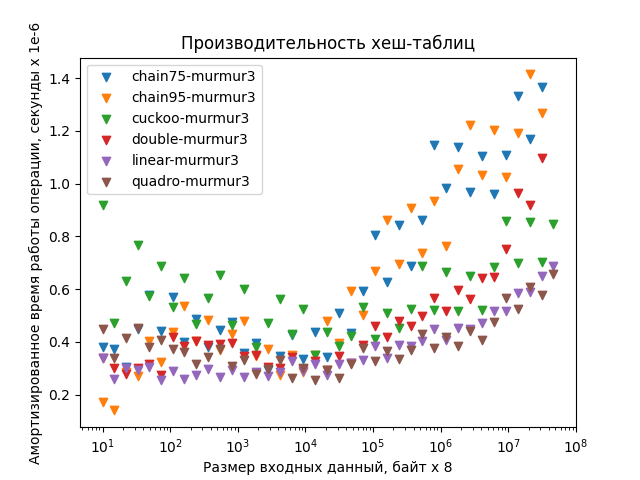
\includegraphics[width=0.8\textwidth]{murmur3-hash-plot.png}
\end{center}

\par
Видно, что таблицы с открытым хешированием и 
линейным и квадратичным пробированием имеют сравнимую эффективность.
Чуть менее эффективна реализация cuckoo-пробирования, а хеш-таблицы,
основанные на методе цепочек для разрешения коллизий имеют худшее время работы
при достаточно большом объеме хранимых данных.

\par
Бенчмарки для различных хеш-функций проводились на реализации с линейным и
cuckoo пробированием.

Линейное пробирование (время измеряется в микросекундах):
\begin{center}
	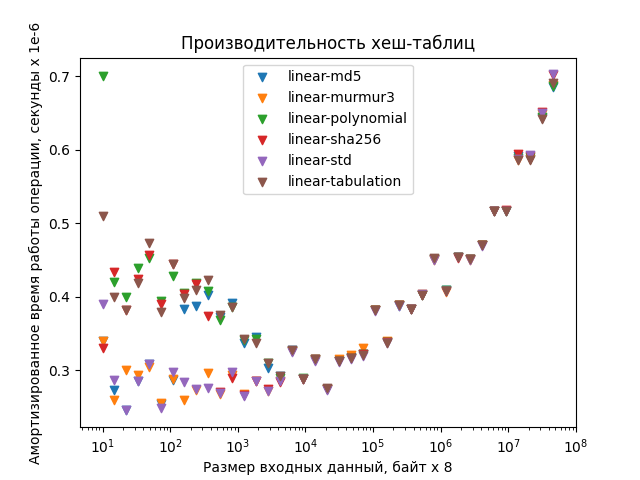
\includegraphics[width=0.8\textwidth]{lineal-table-plot.png}
\end{center}

Cuckoo пробирование (время измеряется в микросекундах):
\begin{center}
	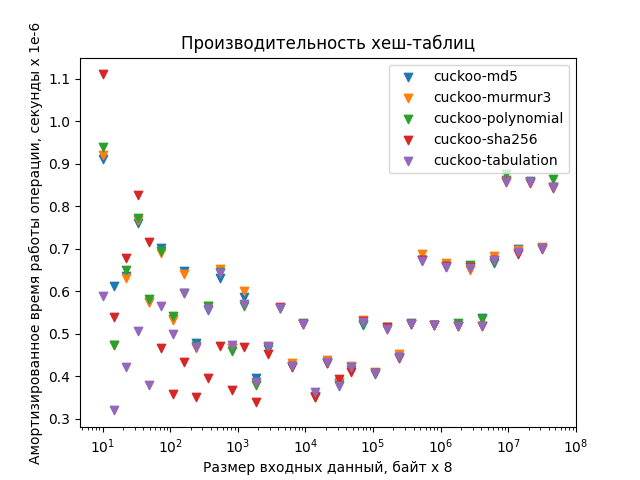
\includegraphics[width=0.8\textwidth]{cuckoo-table-plot.png}
\end{center}

\par
Характерные скачки на графиках могут быть объяснены необходимостью 
затратной операции перехеширования при расширении таблицы.

\subsection{Выводы}
По результатам бенчмарков, на данным порядков размера кеша 2-го и 3-го уровней
лучший результат показывают алгоритмы разрешения коллизий с открытой адресацией
и линейным либо квадратичным пробированием и алгоритмы хеширования 
murmur3 и std::hash в используемой реализации стандартной библиотеки.
Меньшая эффективность cuckoo хеширования может объясняться затратностью
операции вставки и необходимостью использовать две хеш-функции.
Алгоритмы SHA256 и MD5 имеют немного меньшую эффективность из-за избыточной 
длины возвращаемого хеша и большей сложности, обеспечивающей криптографическую
стойкость.

\end{document}
